\hypertarget{page_dmp_sec_dmp_introduction}{}\subsection{Introduction}\label{page_dmp_sec_dmp_introduction}
The core idea behind dynamical movement primitives (D\+M\+Ps) is to represent movement primitives as a combination of dynamical systems (please read \hyperlink{page_dyn_sys}{Dynamical Systems Module}, if you haven't already done so). The state variables of the main dynamical system $ [\mathbf{y \dot{y} \ddot{y}} ]$ then represent trajectories for controlling, for instance, the 7 joints of a robot arm, or its 3\+D end-\/effector position. The attractor state is the end-\/point or {\itshape goal} of the movement.

The key advantage of D\+M\+Ps is that they inherit the nice properties from linear dynamical systems (guaranteed convergence towards the attractor, robustness to perturbations, independence of time, etc) whilst allowing arbitrary (smooth) motions to be represented by adding a non-\/linear forcing term. This forcing term is often learned from demonstration, and subsequently improved through reinforcement learning.

D\+M\+Ps were introduced in {\bfseries [ijspeert02movement]}, but in this section we follow largely the notation and description in {\bfseries [ijspeert13dynamical]}, but at a slower pace.

{\itshape Historical} {\itshape remark}. Recently, the term \char`\"{}dynamic\+A\+L movement primitives\char`\"{} is preferred over \char`\"{}dynamic movement primitives\char`\"{}. The newer term makes the relation to dynamic\+A\+L systems more clear, and avoids confusion about whether the output of \char`\"{}dynamical movement primitives\char`\"{} is in kinematic or dynamic space (it is usually in kinematic space).

{\itshape Remark}. This documentation and code focusses only on discrete movement primitives. For rythmic movement primitives, we refer to {\bfseries [ijspeert13dynamical.]}\hypertarget{page_dmp_sec_core}{}\subsection{Basic Point-\/to-\/\+Point Movements\+: A Critically Damped Spring-\/\+Damper System}\label{page_dmp_sec_core}
At the heart of the D\+M\+P lies a spring-\/damper system, as described in \hyperlink{page_dyn_sys_dyn_sys_spring_damper}{Spring-\/\+Damper Systems}. In D\+M\+P papers, the notation of the spring-\/damper system is usually a bit different\+: \begin{eqnarray*} m\ddot{y} =& -ky -c\dot{y} & \mbox{spring-damper system, ``traditional notation''} \\ m\ddot{y} =& c(-\frac{k}{c}y - \dot{y})\\ \tau\ddot{y} =& \alpha(-\beta y - \dot{y}) & \mbox{with } \alpha=c,~~\beta = \frac{k}{c},~~m=\tau\\ \tau\ddot{y} =& \alpha(-\beta (y-y^g) - \dot{y})& \mbox{with attractor } y^g\\ \tau\ddot{y} =& \alpha(\beta (y^g-y) - \dot{y})& \mbox{typical DMP notation for spring-damper system}\\ \end{eqnarray*}

In the last two steps, we change the attractor state from 0 to $y^g$, where $y^g$ is the goal of the movement.

To avoid overshooting or slow convergence towards $y^g$, we prefer to have a {\itshape critically} {\itshape damped} spring-\/damper system for the D\+M\+P. For such systems $c = 2\sqrt{mk}$ must hold, see \hyperlink{page_dyn_sys_dyn_sys_critical_damping}{Critical Damping}. In our notation this becomes $\alpha = 2\sqrt{\alpha\beta}$, which leads to $\beta = \alpha/4$. This determines the value of $\beta$ for a given value of $\alpha$ in D\+M\+Ps. The influence of $\alpha$ is illustrated in the first figure in \hyperlink{page_dyn_sys_sec_dyn_sys_intro}{Introduction}.

Rewriting the second order dynamical system as a first order system (see \hyperlink{page_dyn_sys_dyn_sys_rewrite_second_first}{Rewriting one 2nd Order Systems as two 1st Order Systems}) with expanded state $ [z~y]$ yields\+:

\begin{eqnarray*} \left[ \begin{array}{l} {\dot{z}} \\ {\dot{y}} \end{array} \right] = \left[ \begin{array}{l} (\alpha (\beta({y}^{g}-{y})-{z}))/\tau \\ {z}/\tau \end{array} \right] \mbox{~~~~with init. state~} \left[ \begin{array}{l} 0 \\ y_0 \end{array} \right] \mbox{~and attr. state~} \left[ \begin{array}{l} {0} \\ {y}^g \end{array} \right] \end{eqnarray*}

Please note that in the implementation, the state is implemented as $ [y~z]$. The order is inconsequential, but we use the notation above ( $[z~y]$) throughout the rest of this tutorial section, for consistency with the D\+M\+P literature.\hypertarget{page_dmp_sec_forcing}{}\subsection{Arbitrary Smooth Movements\+: the Forcing Term}\label{page_dmp_sec_forcing}
The representation described in the previous section has some nice properties in terms of \hyperlink{page_dyn_sys_sec_dyn_sys_convergence}{Convergence towards the Attractor} , \hyperlink{page_dyn_sys_sec_dyn_sys_perturbations}{Robustness to Perturbations} , and \hyperlink{page_dyn_sys_sec_dyn_sys_autonomy}{Autonomy}, but it can only represent very simple movements. To achieve more complex movements, we add a time-\/dependent forcing term to the spring-\/damper system. The spring-\/damper systems and forcing term are together known as a {\itshape transformation} {\itshape system}.

\begin{eqnarray*} \left[ \begin{array}{l} {\dot{z}} \\ {\dot{y}} \end{array} \right] = \left[ \begin{array}{l} (\alpha (\beta({y}^{g}-{y})-{z}) + f(t))/\tau \\ {z}/\tau \end{array} \right] \mbox{~~~~with init. state~} \left[ \begin{array}{l} 0 \\ y_0 \end{array} \right] \mbox{~and attr. state~} \left[ \begin{array}{l} {?} \\ {y}^g \end{array} \right] \end{eqnarray*}

The forcing term is an open loop controller, i.\+e. it depends only on time. By modifying the acceleration profile of the movement with a forcing term, arbitrary smooth movements can be achieved. The function $ f(t)$ is usually a function approximator, such as locally weighted regression (L\+W\+R) or locally weighted projection regression (L\+W\+P\+R), see \hyperlink{page_func_approx}{Function Approximation Module}. The graph below shows an example of a forcing term implemented with L\+W\+R with random weights for the basis functions.


\begin{DoxyImage}
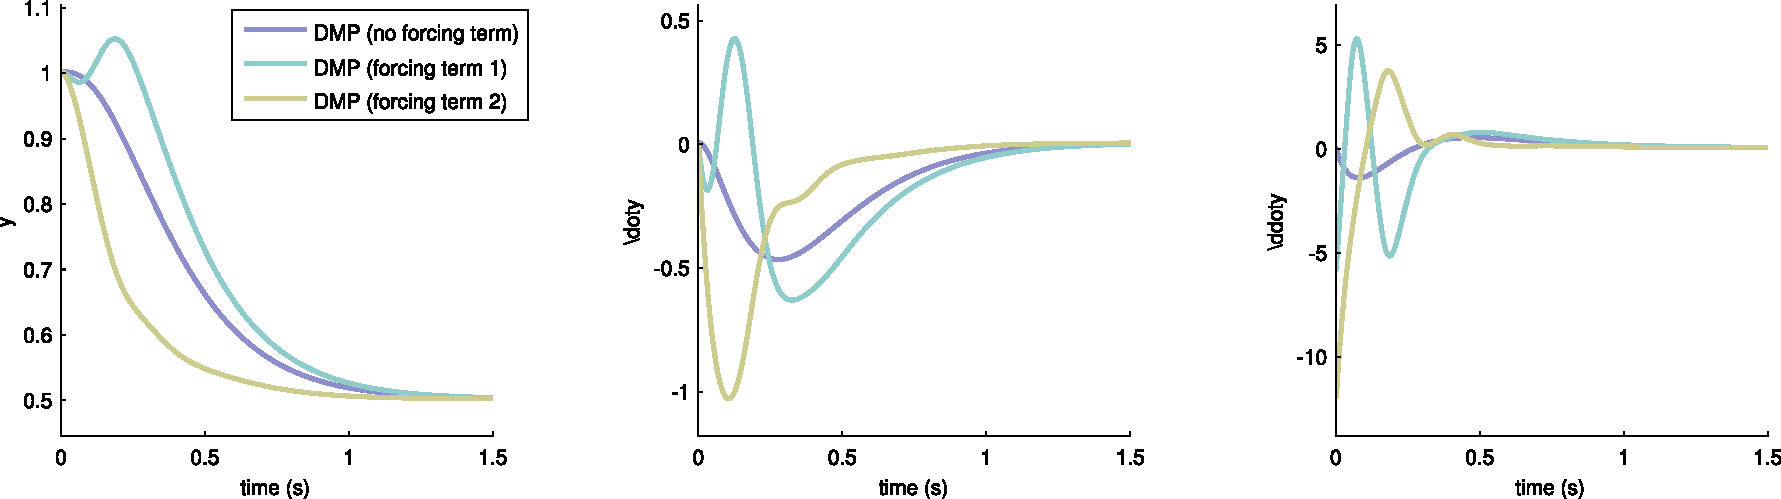
\includegraphics[height=4cm]{dmp_forcing_terms-svg}
\caption{A non-\/linear forcing term enable more complex trajectories to be generated (these D\+M\+Ps use a goal system and an exponential gating term).}
\end{DoxyImage}
\hypertarget{page_dmp_sec_forcing_convergence}{}\subsubsection{Ensuring Convergence to 0 of the Forcing Term\+: the Gating System}\label{page_dmp_sec_forcing_convergence}
Since we add a forcing term to the dynamical system, we can no longer guarantee that the system will converge towards $ x^g $; perhaps the forcing term continually pushes it away $ x^g $ (perhaps it doesn't, but the point is that we cannot {\itshape guarantee} that it {\itshape always} doesn't). That is why there is a question mark in the attractor state in the equation above. To guarantee that the movement will always converge towards the attractor $ x^g $, we need to ensure that the forcing term decreases to 0 towards the end of the movement. To do so, a gating term is added, which is 1 at the beginning of the movement, and 0 at the end. This gating term itself is determined by, of course, a dynamical system. In {\bfseries [ijspeert02movement]}, it was suggested to use an exponential system. We add this extra system to our dynamical system by expanding the state as follows\+:

\begin{eqnarray*} \dot{x} = \left[ \begin{array}{l} {\dot{z}} \\ {\dot{y}} \\ {\dot{x}} \end{array} \right] = \left[ \begin{array}{l} (\alpha_y (\beta_y({y}^{g}-{y})-{z}) + x\cdot f(t))/\tau \\ {z}/\tau \\ -\alpha_x x/\tau \end{array} \right] \mbox{~~~~with init. state~} \left[ \begin{array}{l} 0 \\ y_0 \\ 1 \end{array} \right] \mbox{~and attr. state~} \left[ \begin{array}{l} {0} \\ {y}^g \\ 0 \end{array} \right] \end{eqnarray*}\hypertarget{page_dmp_sec_forcing_autonomy}{}\subsubsection{Ensuring Autonomy of the Forcing Term\+: the Phase System}\label{page_dmp_sec_forcing_autonomy}
By introducing the dependence of the forcing term $ f(t)$ on time $ t $ the overall system is no longer autonomous. To achieve independence of time, we therefore let $ f $ be a function of the state of an (autonomous) dynamical system rather than of $ t $. This system represents the {\itshape phase} of the movement. {\bfseries [ijspeert02movement]} suggested to use the same dynamical system for the gating and phase, and use the term {\itshape canonical} {\itshape system} to refer this joint gating/phase system. Thus the phase of the movement starts at 1, and converges to 0 towards the end of the movement, just like the gating system. The new formulation now is (the only difference is $ f(x)$ instead of $ f(t)$)\+:

\begin{eqnarray*} \left[ \begin{array}{l} {\dot{z}} \\ {\dot{y}} \\ {\dot{x}} \end{array} \right] = \left[ \begin{array}{l} (\alpha_y (\beta_y({y}^{g}-{y})-{z}) + x\cdot f(x))/\tau \\ {z}/\tau \\ -\alpha_x x/\tau \end{array} \right] \mbox{~~~~with init. state~} \left[ \begin{array}{l} 0 \\ y_0 \\ 1 \end{array} \right] \mbox{~and attr. state~} \left[ \begin{array}{l} {0} \\ {y}^g \\ 0 \end{array} \right] \end{eqnarray*}

\begin{DoxyRefDesc}{Todo}
\item[\hyperlink{todo__todo000006}{Todo}]Discuss goal-\/dependent scaling, i.\+e. $ f(t)s(x^g-x_0) $?\end{DoxyRefDesc}
\hypertarget{page_dmp_sec_multidim_dmp}{}\subsubsection{Multi-\/dimensional Dynamic Movement Primitives}\label{page_dmp_sec_multidim_dmp}
Since D\+M\+Ps usually have multi-\/dimensional states (e.\+g. one output $ {\mathbf{y}}_{d=1\dots D}$ for each of the $ D $ joints), it is more accurate to use bold fonts for the state variables (except the gating/phase system, because it is always 1\+D) so that they represent vectors\+:

\begin{eqnarray*} \left[ \begin{array}{l} {\dot{\mathbf{z}}} \\ {\dot{\mathbf{y}}} \\ {\dot{x}} \end{array} \right] = \left[ \begin{array}{l} (\alpha_y (\beta_y({\mathbf{y}}^{g}-\mathbf{y})-\mathbf{z}) + x\cdot f(x))/\tau \\ \mathbf{z}/\tau \\ -\alpha_x x/\tau \end{array} \right] \mbox{~~~~with init. state~} \left[ \begin{array}{l} \mathbf{0} \\ \mathbf{z}_0 \\ 1 \end{array} \right] \mbox{~and attr. state~} \left[ \begin{array}{l} \mathbf{0} \\ \mathbf{y}^g \\ 0 \end{array} \right] \end{eqnarray*}

So far, the graphs have shown 1-\/dimensional systems. To generate D-\/dimensional trajectories for, for instance, the 7 joints of an arm or the 3\+D position of its end-\/effector, we simply use D transformation systems. A key principle in D\+M\+Ps is to use one and the same phase system for all of the transformation systems, to ensure that the output of the transformation systems are synchronized in time. The image below show the evolution of all the dynamical systems involved in integrating a multi-\/dimensional D\+M\+P.


\begin{DoxyImage}
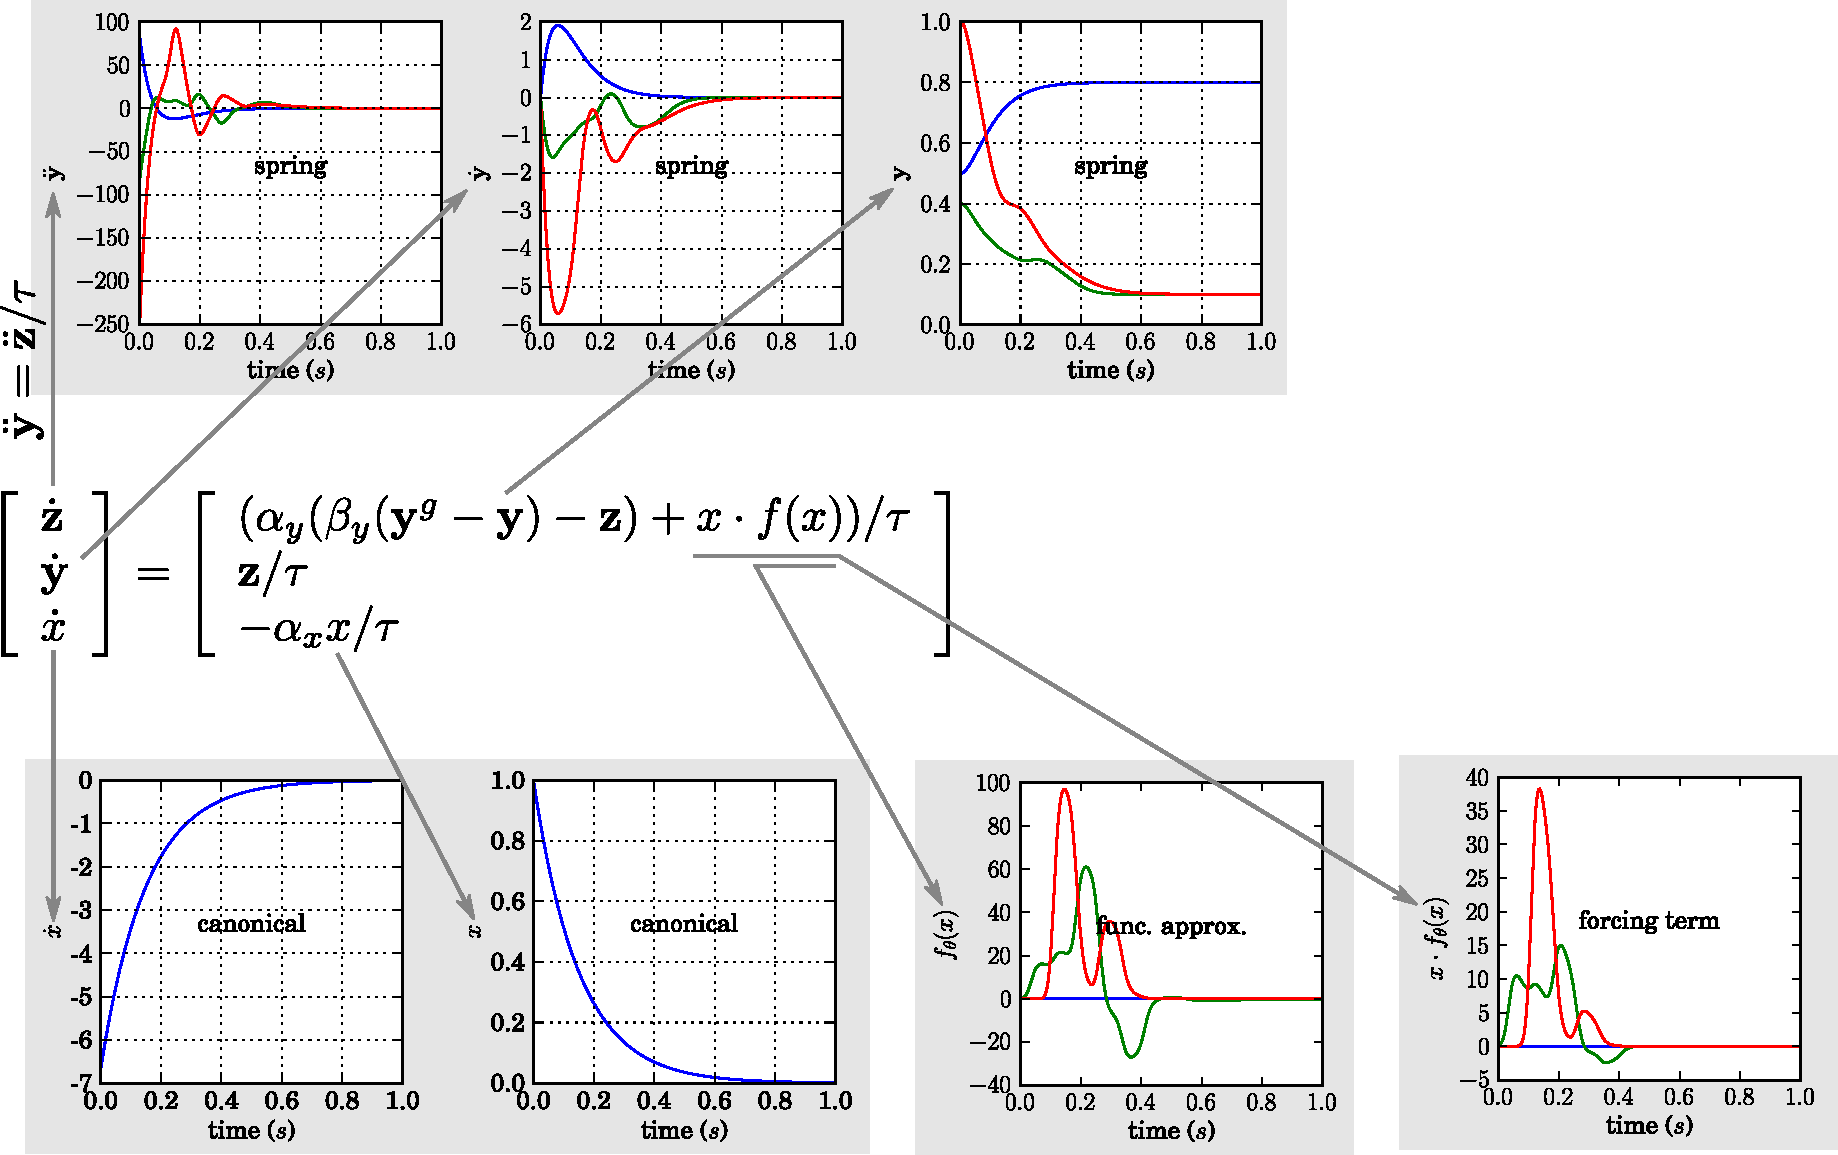
\includegraphics[height=8cm]{dmpplot_ijspeert2002movement-svg}
\caption{The various dynamical systems and forcing terms in multi-\/dimensional D\+M\+Ps.}
\end{DoxyImage}


{\itshape }

{\itshape }\hypertarget{page_dyn_sys_Implementation}{}\subsubsection{Implementation}\label{page_dyn_sys_Implementation}
{\itshape  Since a Dynamical Movement Primitive is a dynamical system, the Dmp class derives from the Dynamical\+System class. It overrides the virtual function Dynamical\+System\+::integrate\+Start(). Integrating the D\+M\+P numerically (Euler or 4th order Runge-\/\+Kutta) is done with the generic Dynamical\+System\+::integrate\+Step() function. It also implements the pure virtual function Dynamical\+System\+::analytical\+Solution(). Because a D\+M\+P cannot be solved analytically (we cannot write it in closed form due to the arbitrary forcing term), calling Dmp\+::analytical\+Solution() in fact performs a numerical Euler integration (although the linear subsystems (phase, gating, etc.) are analytically solved because this is faster computationally).}

{\itshape Please note that in this tutorial we have used the notation $[z~y]$ for consistency with the D\+M\+P literature. In the C++ implementation, the order is rather $[y~z]$.}

{\itshape {\itshape Remark}. Dmp inherits the function Dynamical\+System\+::integrate\+Step() from the Dynamical\+System class. Dynamical\+System\+::integrate\+Step() uses either Euler integration, or 4-\/th order Runge-\/\+Kutta. The latter is more accurate, but requires 4 calls of Dynamical\+System\+::differential\+Equation() instead of 1). Which one is used can be set with Dynamical\+System\+::set\+\_\+integration\+\_\+method(). To numerically integrate a dynamical system, one must carefully choose the integration time dt. Choosing it too low leads to inaccurate integration, and the numerical integration will diverge from the 'true' solution acquired through analytical solution. See \href{http://en.wikipedia.org/wiki/Euler%27s_method}{\tt http\+://en.\+wikipedia.\+org/wiki/\+Euler\%27s\+\_\+method} for examples. Choosing dt depends entirely on the time-\/scale (seconds vs. years) and parameters of the dynamical system (time constant, decay parameters). For D\+M\+Ps, which are expected to take between 0.\+5-\/10 seconds, dt is usually chosen to be in the range 0.\+01-\/0.\+001. }\hypertarget{page_dmp_sec_dmp_alternative}{}\subsection{Alternative Systems for Gating, Phase and Goals}\label{page_dmp_sec_dmp_alternative}
\hypertarget{page_dmp_sec_dmp_sigmoid_gating}{}\subsubsection{Gating\+: Sigmoid System}\label{page_dmp_sec_dmp_sigmoid_gating}
A disadvantage of using an exponential system as a gating term is that the gating decreases very quickly in the beginning. Thus, the output of the function approximator $ f(x) $ needs to be very high towards the end of the movement if it is to have any effect at all. This leads to scaling issues when training the function approximator.

Therefore, sigmoid systems have more recently been proposed {\bfseries [kulvicius12joining]} as a gating system. This leads to the following D\+M\+P formulation (since the gating and phase system are no longer shared, we introduce a new state variable $ v $ for the gating term\+:

\begin{eqnarray*} \left[ \begin{array}{l} {\dot{\mathbf{z}}} \\ {\dot{\mathbf{y}}} \\ {\dot{x}} \\ {\dot{v}} \end{array} \right] = \left[ \begin{array}{l} (\alpha_y (\beta_y({\mathbf{y}}^{g}-\mathbf{y})-\mathbf{z}) + v\cdot f(x))/\tau \\ \mathbf{z}/\tau \\ -\alpha_x x/\tau \\ -\alpha_v v (1-v/v_{\mbox{\scriptsize max}}) \end{array} \right] \mbox{~~~~with init. state~} \left[ \begin{array}{l} \mathbf{0} \\ \mathbf{y}_0 \\ 1 \\ 1 \end{array} \right] \mbox{~and attr. state~} \left[ \begin{array}{l} \mathbf{0} \\ \mathbf{y}^g \\ 0 \\ 0 \end{array} \right] \end{eqnarray*}

where the term $ v_{\mbox{\scriptsize max}}$ is determined by $\tau $\hypertarget{page_dmp_sec_dmp_phase}{}\subsubsection{Phase\+: Constant Velocity System}\label{page_dmp_sec_dmp_phase}
In practice, using an exponential phase system may complicate imitation learning of the function approximator $ f $, because samples are not equidistantly spaced in time. Therefore, we introduce a dynamical system that mimics the properties of the phase system described in {\bfseries [kulvicius12joining]}, whilst allowing for a more natural integration in the D\+M\+P formulation, and thus our code base. This system starts at 0, and has a constant velocity of $1/\tau$, which means the system reaches 1 when $t=\tau$. When this point is reached, the velocity is set to 0.

\begin{eqnarray*} \dot{x} =& 1/\tau \mbox{~if~} x < 1 & \\ & 0 \mbox{~if~} x>1 \\ \end{eqnarray*}

This, in all honesty, is a bit of a hack, because it leads to a non-\/smooth acceleration profile. However, its properties as an input to the function approximator are so advantageous that we have designed it in this way (the implementation of this system is in the Time\+System class).


\begin{DoxyImage}
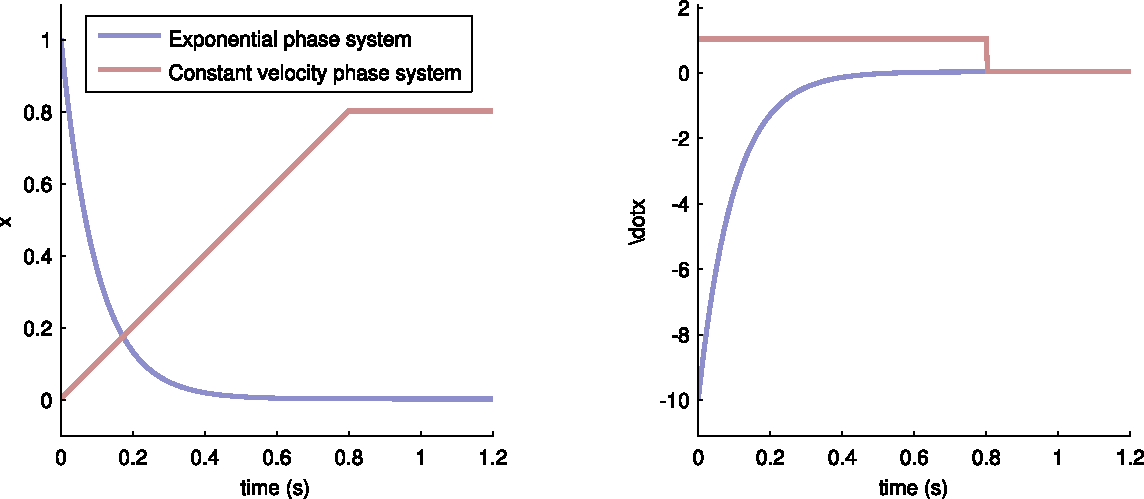
\includegraphics[height=4cm]{phase_systems-svg}
\caption{Exponential and constant velocity dynamical systems as the 1\+D phase for a dynamical movement primitive.}
\end{DoxyImage}


With the constant velocity dynamical system the D\+M\+P formulation becomes\+:

\begin{eqnarray*} \left[ \begin{array}{l} {\dot{\mathbf{z}}} \\ {\dot{\mathbf{y}}} \\ {\dot{x}} \\ {\dot{v}} \end{array} \right] = \left[ \begin{array}{l} (\alpha_y (\beta_y({\mathbf{y}}^{g}-\mathbf{y})-\mathbf{z}) + v\cdot f(x))/\tau \\ \mathbf{z}/\tau \\ 1/\tau \\ -\alpha_v v (1-v/v_{\mbox{\scriptsize max}}) \end{array} \right] \mbox{~~~~with init. state~} \left[ \begin{array}{l} \mathbf{0} \\ \mathbf{y}_0 \\ 0 \\ 1 \end{array} \right] \mbox{~and attr. state~} \left[ \begin{array}{l} \mathbf{0} \\ \mathbf{y}^g \\ 1 \\ 0 \end{array} \right] \end{eqnarray*}\hypertarget{page_dmp_sec_delayed_goal}{}\subsubsection{Zero Initial Accelerations\+: the Delayed Goal System}\label{page_dmp_sec_delayed_goal}
Since the spring-\/damper system leads to high initial accelerations (see the graph to the right below), which is usually not desirable for robots, it was suggested to move the attractor of the system from the initial state $ y_0 $ to the goal state $ y^g $ {\itshape during} the movement {\bfseries [kulvicius12joining.]} This delayed goal attractor $ y^{g_d} $ itself is represented as an exponential dynamical system that starts at $ y_0 $, and converges to $ y^g $ (in early versions of D\+M\+Ps, there was no delayed goal system, and $ y^{g_d} $ was simply equal to $ y^g $ throughout the movement). The combination of these two systems, listed below, leads to a movement that starts and ends with 0 velocities and accelerations, and approximately has a bell-\/shaped velocity profile. This representation is thus well suited to generating human-\/like point-\/to-\/point movements, which have similar properties.

\begin{eqnarray*} \left[ \begin{array}{l} {\dot{\mathbf{z}}} \\ {\dot{\mathbf{y}}} \\ {\dot{\mathbf{y}}^{g_d}} \\ {\dot{x}} \\ {\dot{v}} \end{array} \right] = \left[ \begin{array}{l} (\alpha_y (\beta_y({\mathbf{y}}^{g_d}-\mathbf{y})-\mathbf{z}) + v\cdot f(x))/\tau \\ \mathbf{z}/\tau \\ -\alpha_g({\mathbf{y}^g-\mathbf{y}^{g_d}}) \\ 1/\tau \\ -\alpha_v v (1-v/v_{\mbox{\scriptsize max}}) \end{array} \right] \mbox{~~~~with init. state~} \left[ \begin{array}{l} \mathbf{0} \\ \mathbf{y}_0 \\ \mathbf{y}_0 \\ 0 \\ 1 \end{array} \right] \mbox{~and attr. state~} \left[ \begin{array}{l} \mathbf{0} \\ \mathbf{y}^g \\ \mathbf{y}^g \\ 1 \\ 0 \end{array} \right] \end{eqnarray*}


\begin{DoxyImage}
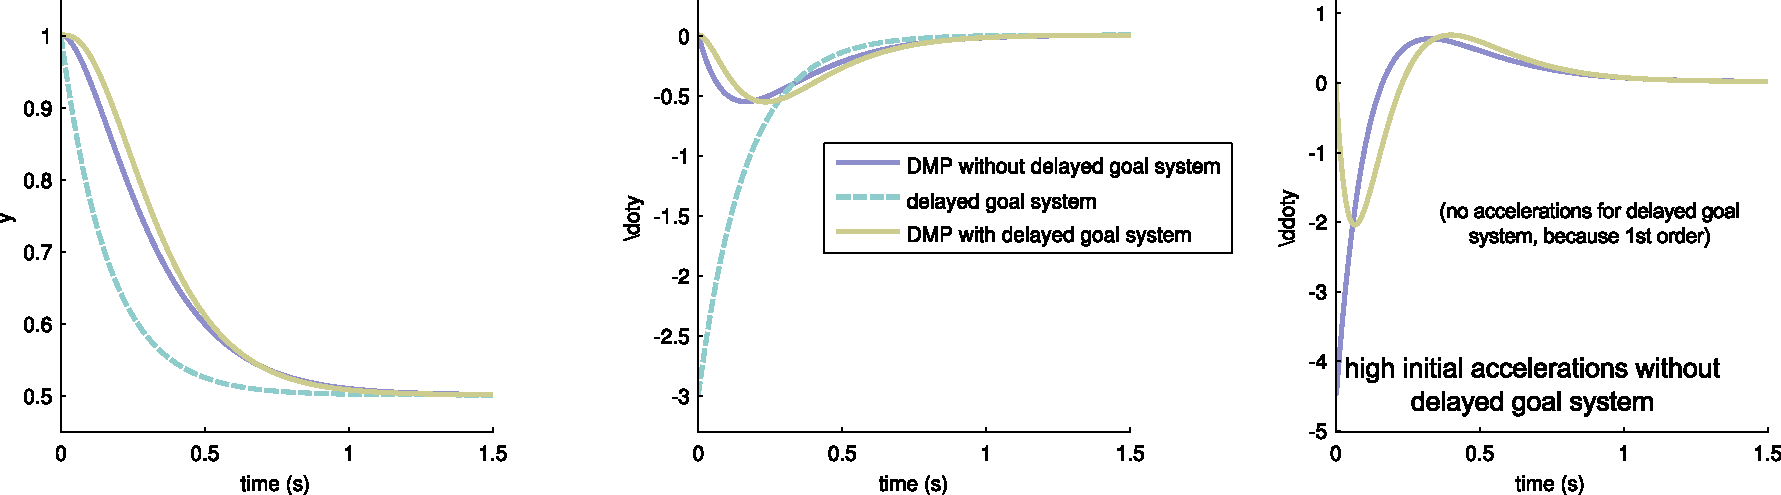
\includegraphics[height=4cm]{dmp_and_goal_system-svg}
\caption{A first dynamical movement primitive, with and without a delayed goal system (left\+: state variable, center\+: velocities, right\+: accelerations.}
\end{DoxyImage}


In my experience, this D\+M\+P formulation is the best for learning human-\/like point-\/to-\/point movements (bell-\/shaped velocity profile, approximately zero velocities and accelerations at beginning and start of the movement), and generates nice normalized data for the function approximator without scaling issues (an exact empirical evaluation is on the stack...). The image below shows the interactions between the spring-\/damper system, delayed goal system, phase system and gating system.


\begin{DoxyImage}
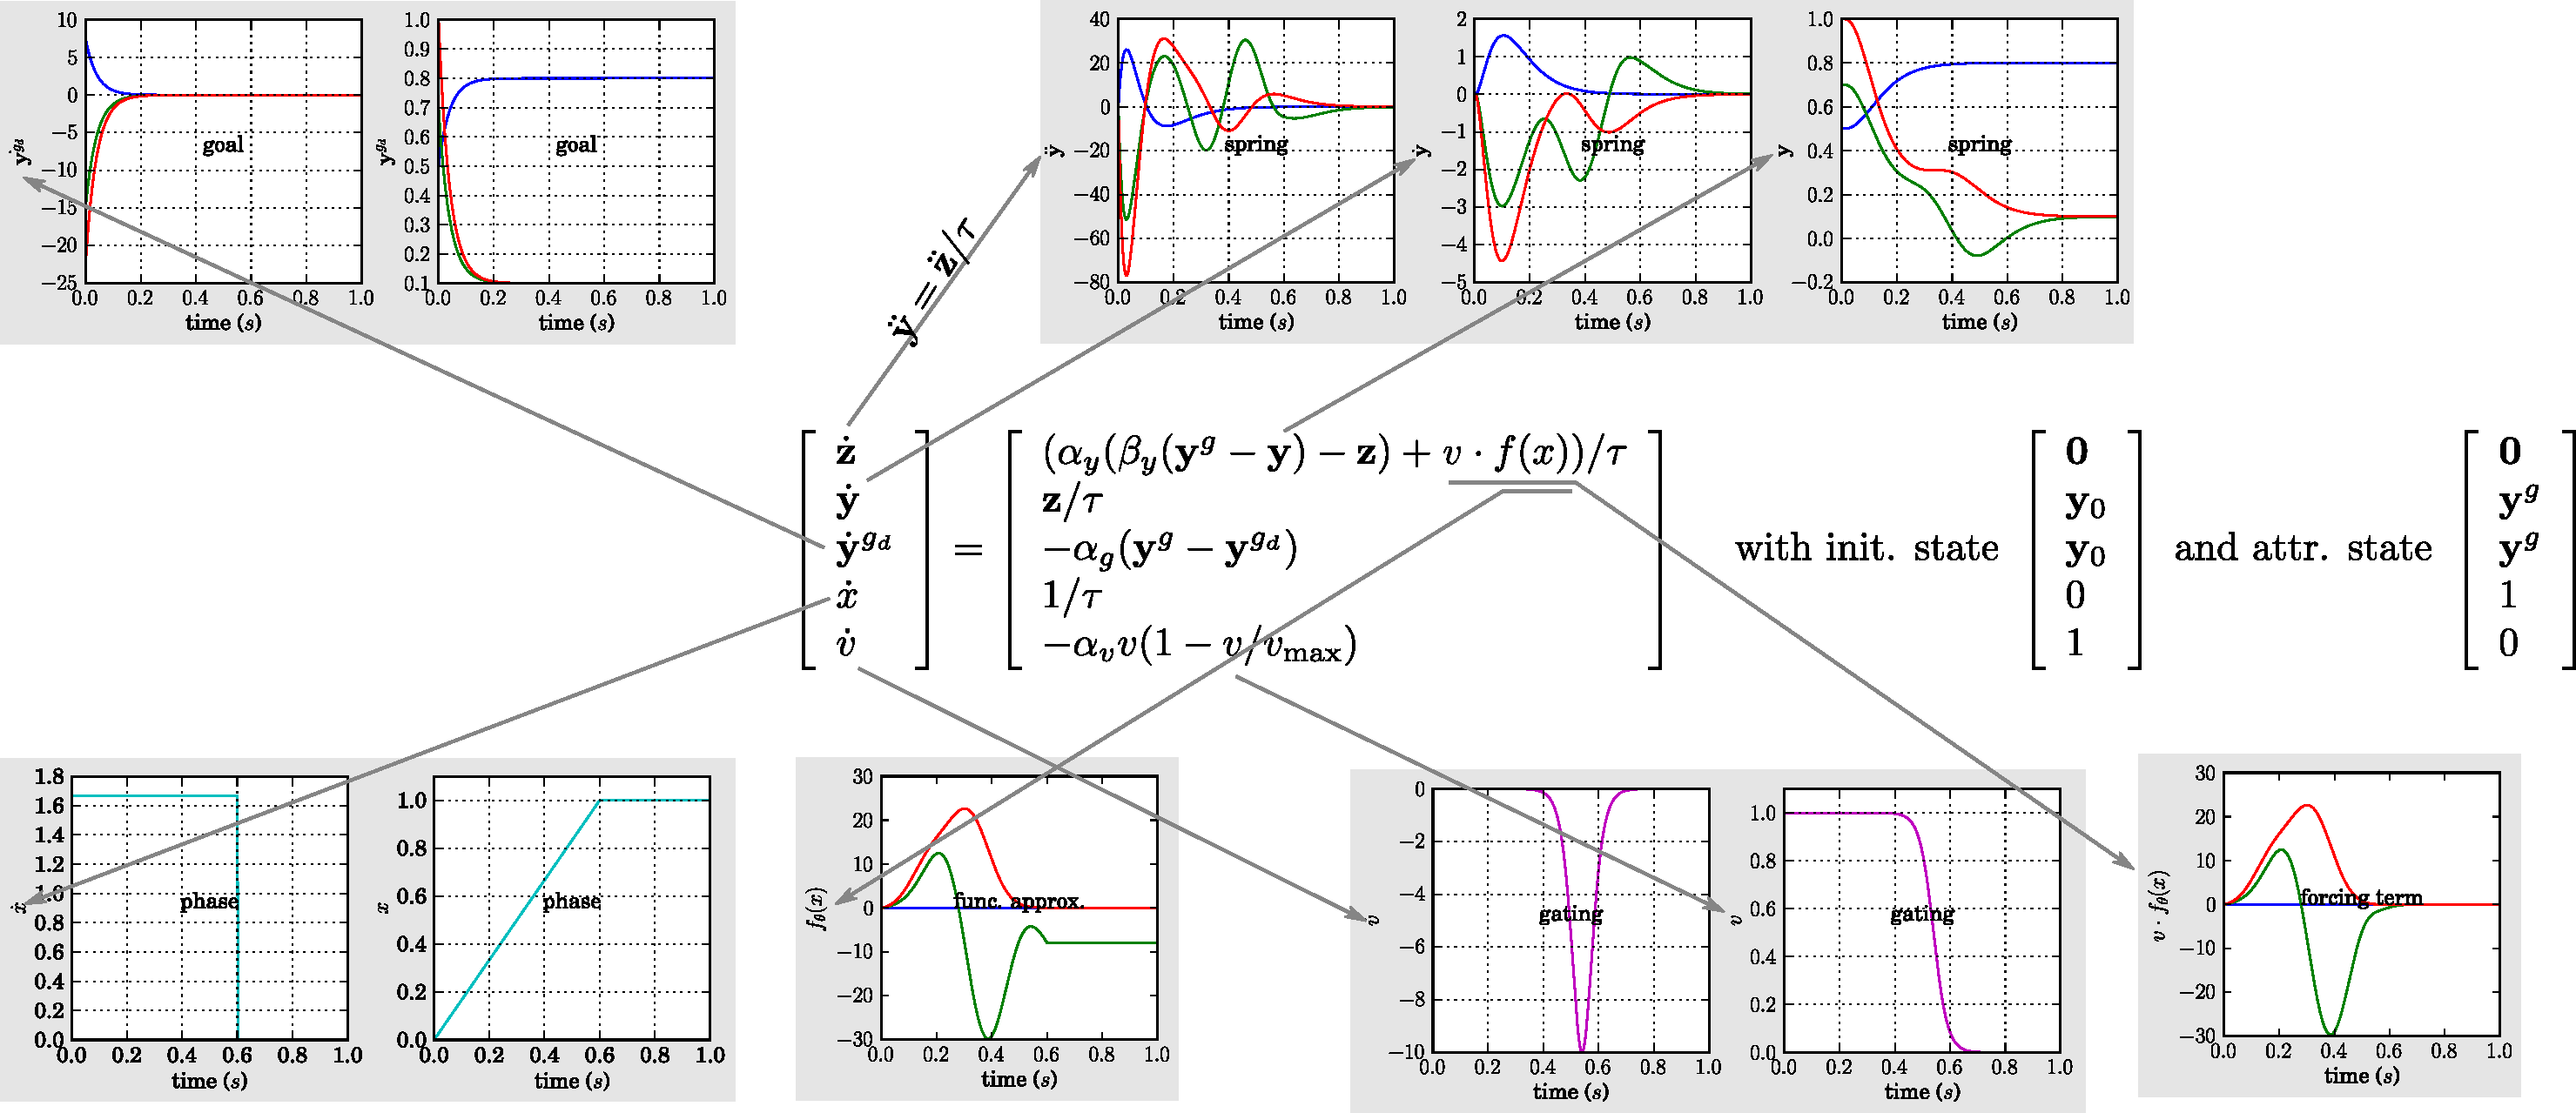
\includegraphics[height=7cm]{dmpplot_kulvicius2012joining-svg}
\caption{The various dynamical systems and forcing terms in multi-\/dimensional D\+M\+Ps.}
\end{DoxyImage}
\hypertarget{page_dmp_sec_dmp_issues}{}\subsection{Known Issues}\label{page_dmp_sec_dmp_issues}
\begin{DoxyRefDesc}{Todo}
\item[\hyperlink{todo__todo000007}{Todo}]Known Issues\end{DoxyRefDesc}


\begin{DoxyItemize}
\item Scaling towards novel goals\end{DoxyItemize}
\hypertarget{page_dmp_sec_dmp_summary}{}\subsection{Summary}\label{page_dmp_sec_dmp_summary}
The core idea in dynamical movement primitives is to combine dynamical systems, which have nice properties in terms of convergence towards the goal, robustness to perturbations, and independence of time, with function approximators, which allow for the generation of arbitrary (smooth) trajectories. The key enabler to this approach is to gate the output of the function approximator with a gating system, which is 1 at the beginning of the movement, and 0 towards the end.

Further enhancements can be made by making the system autonomous (by using the output of a phase system rather than time as an input to the function approximator), or having initial velocities and accelerations of 0 (by using a delayed goal system).

Multi-\/dimensional D\+M\+Ps are achieved by using multi-\/dimensional dynamical systems, and learning one function approximator for each dimension. Synchronization of the different dimensions is ensure by coupling them with only {\itshape one} phase system. 